\begin{tcolorbox}
In diesem Kapitel werden erste Skizzen (Mockups) der Benutzeroberflächen dargestellt.
Diese sollen in erster Linie dazu dienen, dem Kunden einen Überblick über die zu erstellenden UIs zu geben und ggf. Änderungen frühzeitig durchführen zu können.
Dafür eignen sich spezielle Tools, wie z.B. Balsamiq Mockups\footnote{\url{https://balsamiq.com/products/mockups}}.
\end{tcolorbox}


\begin{figure}[h]
\begin{tabularx}{\textwidth}{X  X}
	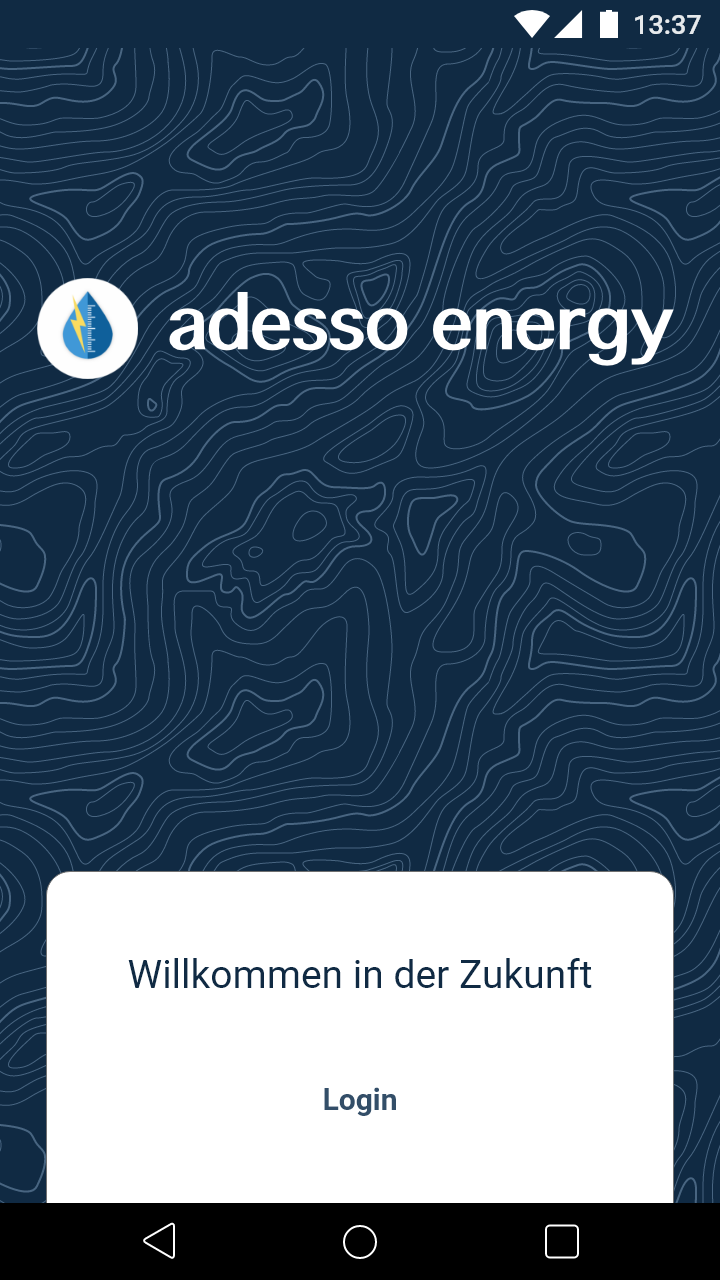
\includegraphics[scale = 0.155]{img/AndroidMockup/splash}  \caption {Startbildschirm} &  Dies ist der Bildschirm, den der Benutzer sieht, sobald er die App startet und noch nicht eingeloggt war.\\
	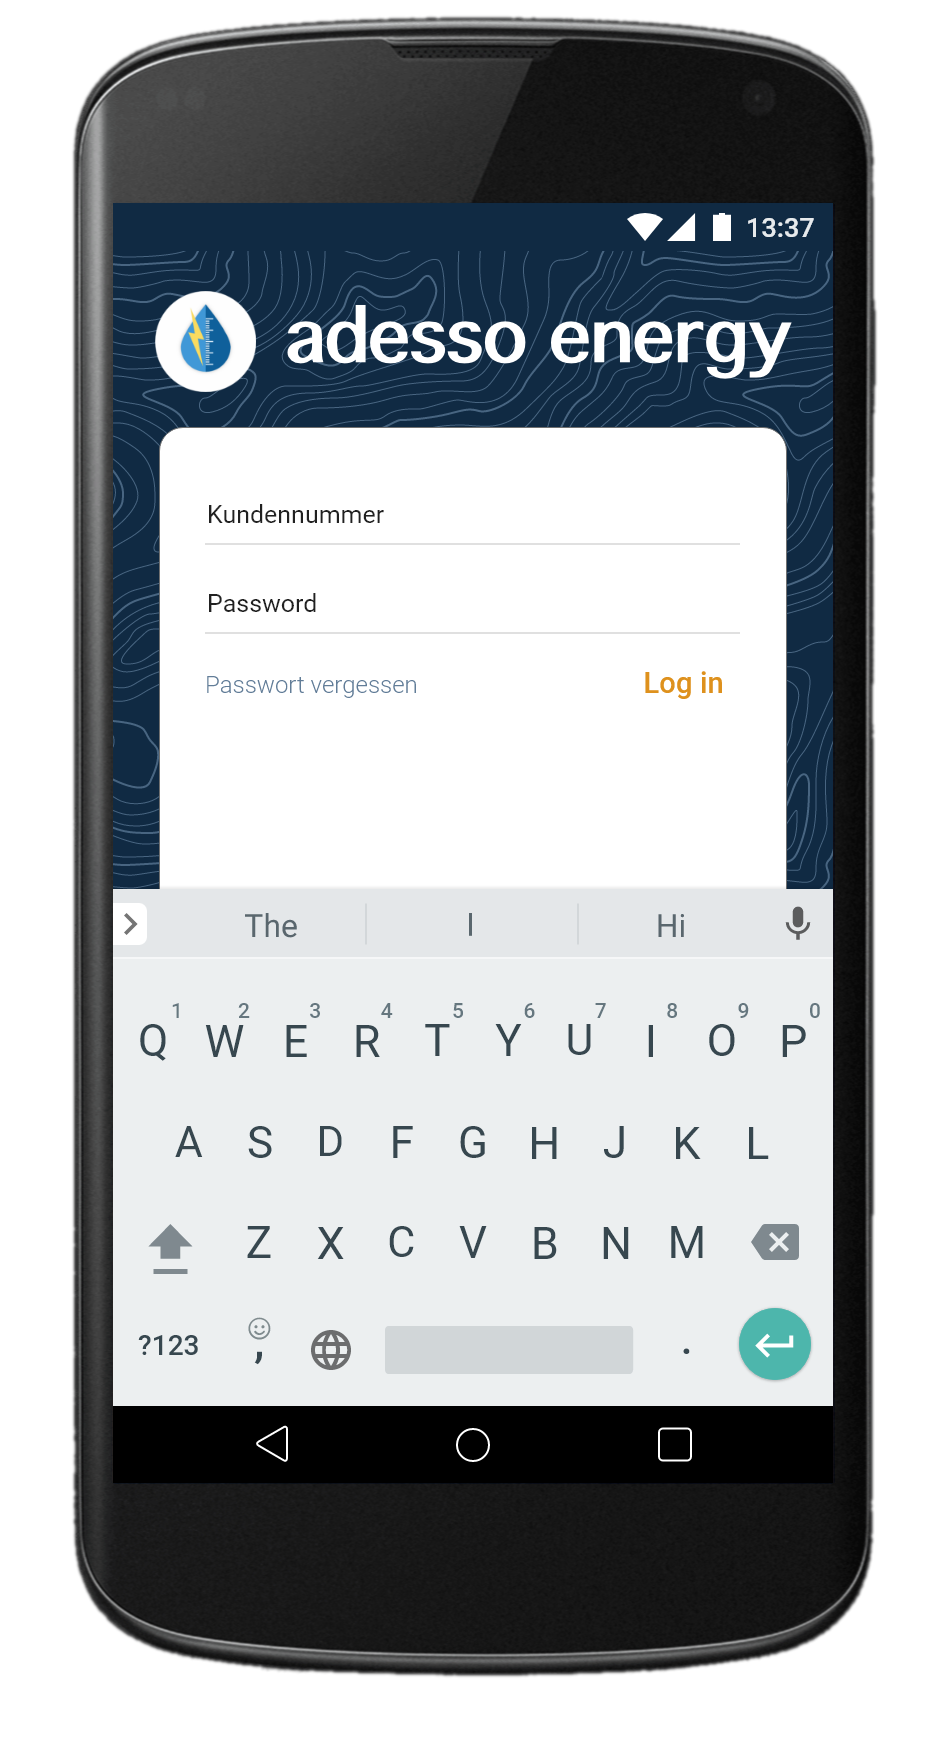
\includegraphics[scale = 0.155]{img/AndroidMockup/login} \caption {Anmeldebildschirm} &	Nachdem man auf dem Startbildschirm auf 'Log in' gedrückt hat, wird man auf den Anmeldebildschirm geleitet. Hier hat man die Möglichkeit, sich mit seiner Kundennummer und seinem Passwort einzuloggen. Außerdem hat man die Möglichkeit, mithilfe des 'Passwort vergessen'-Buttons, sein Passwort zurückzusetzen. \\ 
\end{tabularx}
\end{figure}


\begin{figure}[h]
\begin{tabularx}{\textwidth}{X  X}
	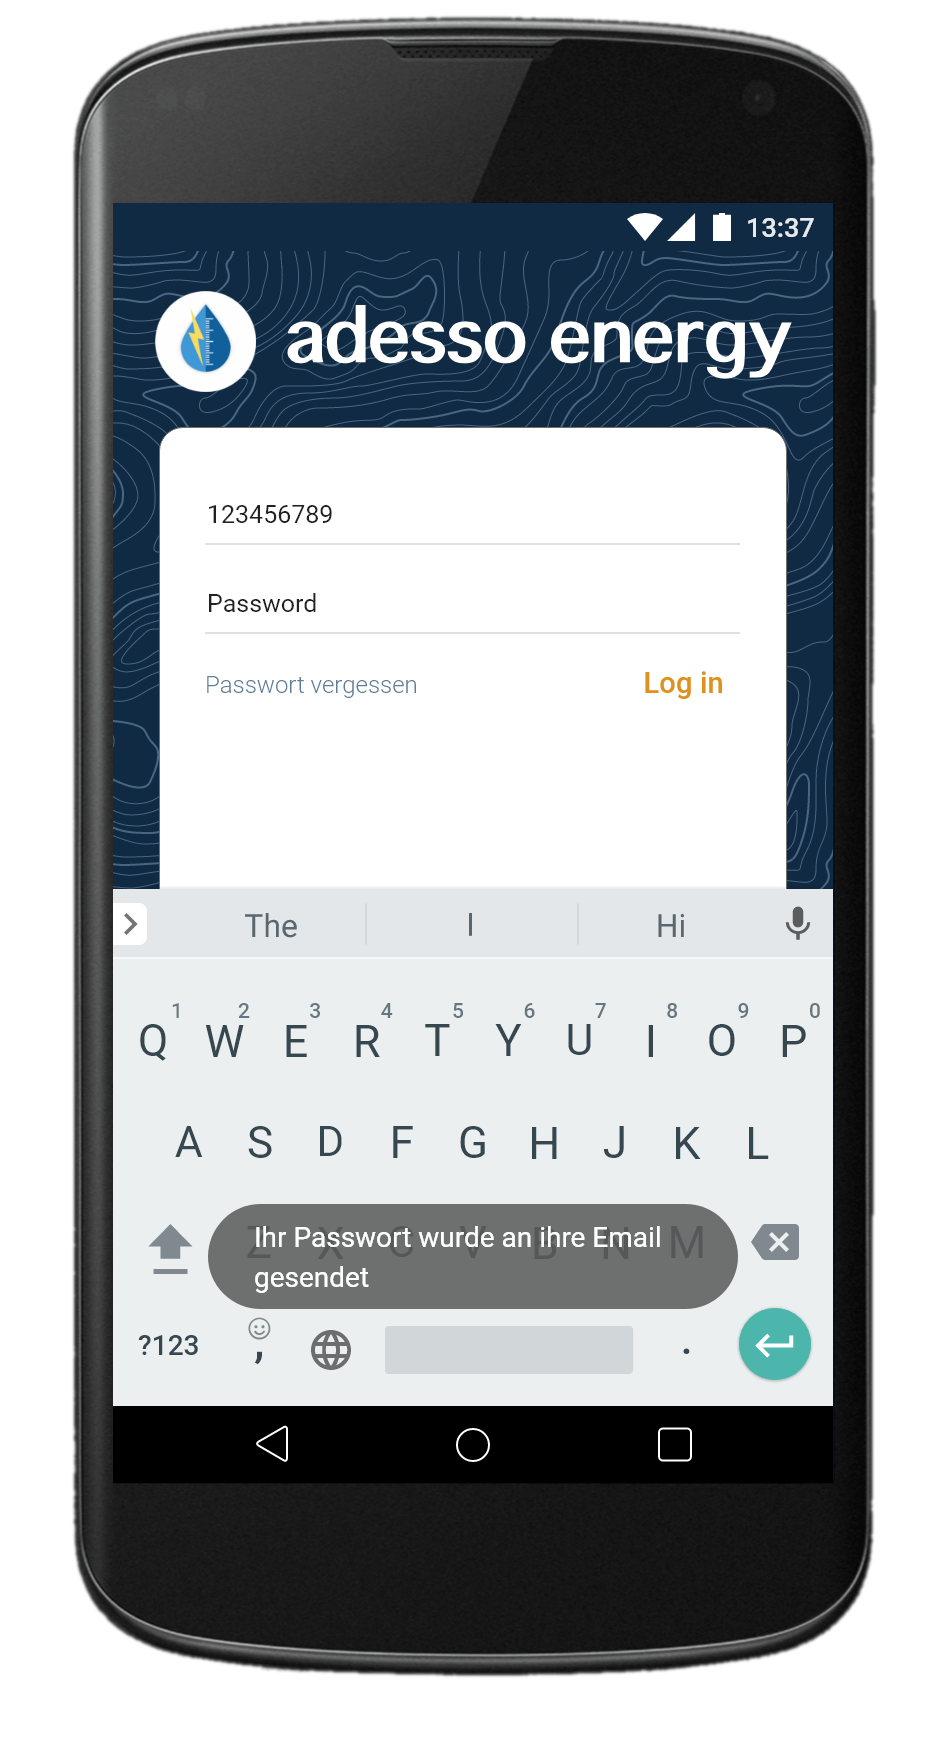
\includegraphics[scale = 0.155]{img/AndroidMockup/forgotPassword} \caption{Password vergessen} & Nachdem man auf 'Passwort vergessen' geklickt hat, erscheint eine Meldung, welche den Benutzer über das weitere Vorgehen informiert.\\
	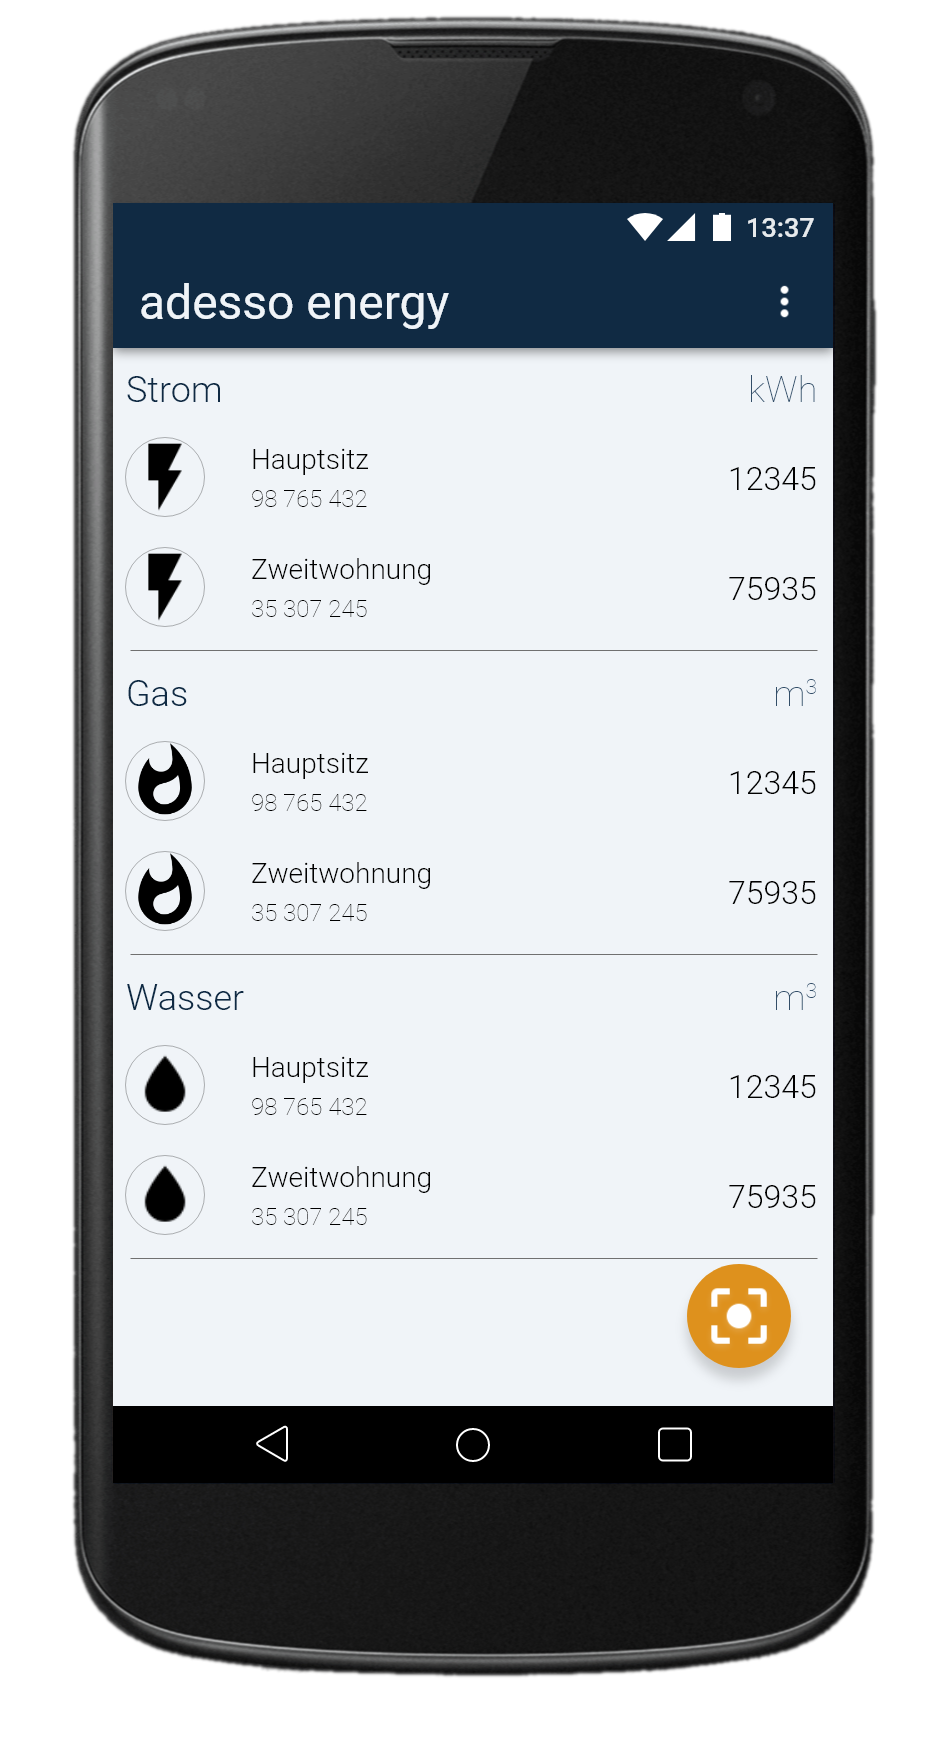
\includegraphics[scale = 0.155]{img/AndroidMockup/Main} \caption{Hauptbildschirm} & Nachdem man sich erfolgreich eingeloggt hat, landet man auf dem Hauptbildschirm. Hier sieht man eine Übersicht seiner Zähler mit deren Zählernummer und aktuellem Zählerstand. \\
\end{tabularx}
\end{figure}


\begin{figure}[h]
\begin{tabularx}{\textwidth}{X  X}
	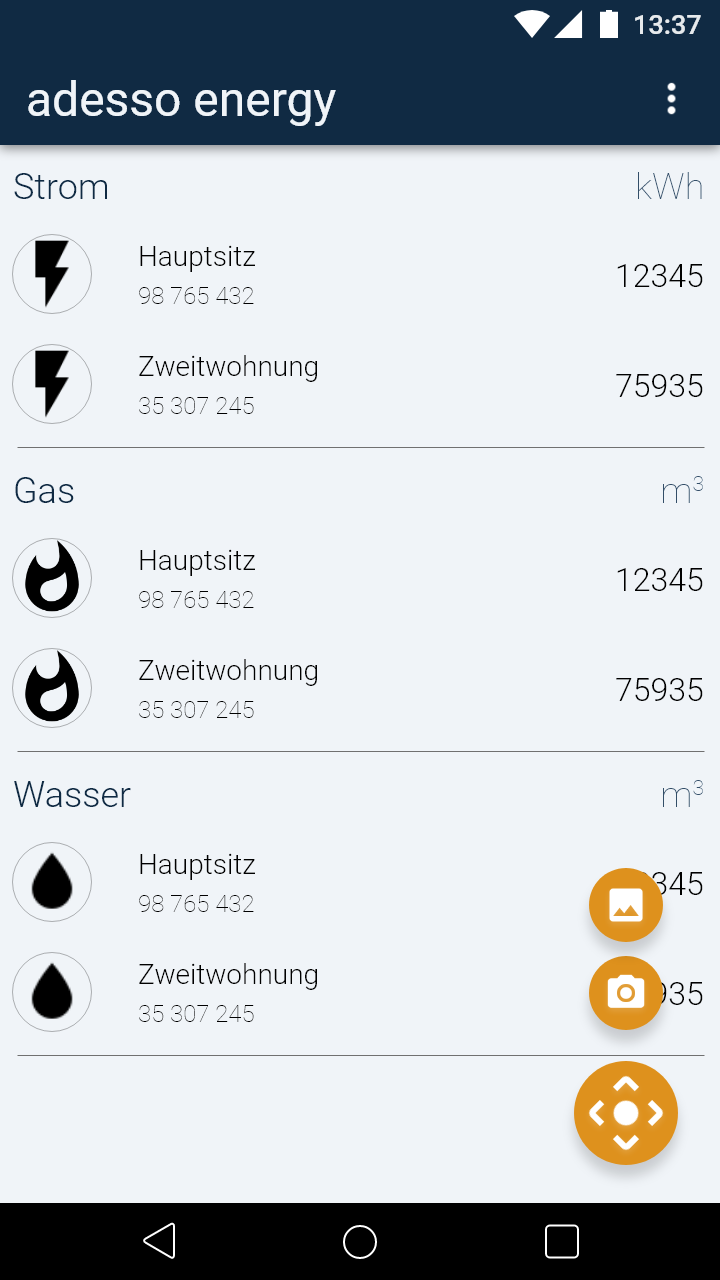
\includegraphics[scale = 0.155]{img/AndroidMockup/FABMenu} \caption{FAB-Menü}  & Klickt man auf den FAB, so erscheint ein Menü. Hier kann man sich entscheiden, ob man ein Bild aufnehmen möchte (Kamera-Symbol) oder eines aus der Galerie hochladen möchte (Galerie-Symbol). \\
	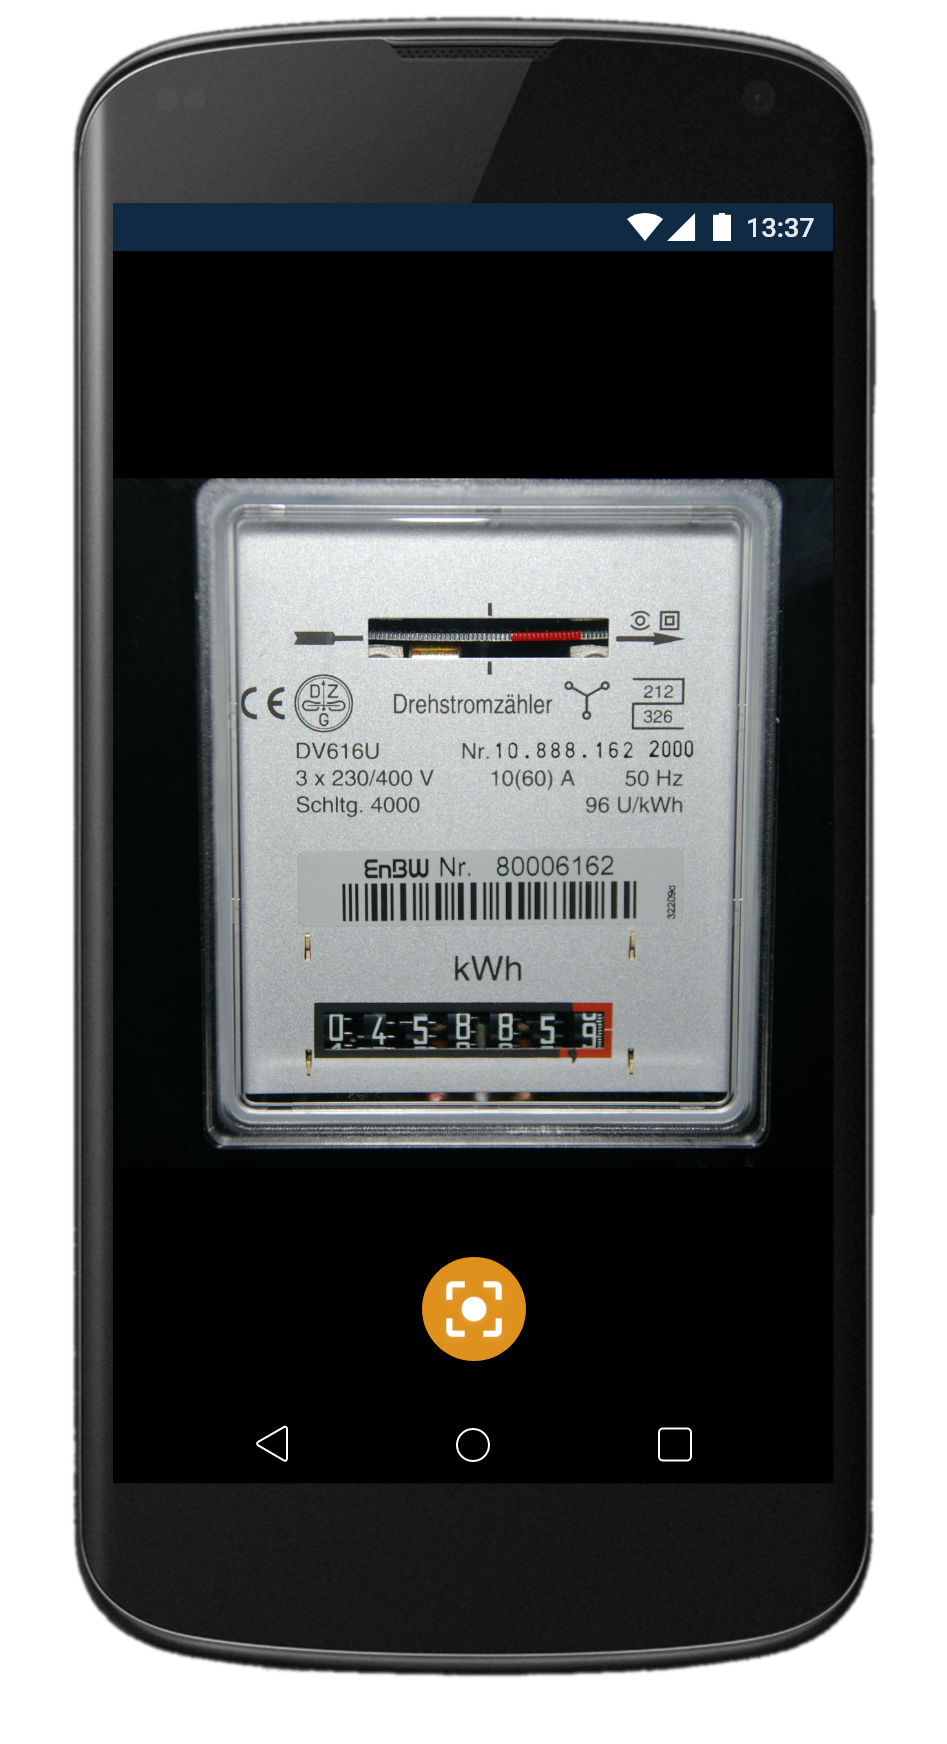
\includegraphics[scale = 0.155]{img/AndroidMockup/SystemCamera} \caption{Kamera-View}  & Nachdem man im Dropdown Menü das Kamera-Symbol gedrückt hat, öffnet sich die Kamera-App des Gerätes. \\ 
\end{tabularx}
\end{figure}

\begin{figure}[h]
\begin{tabularx}{\textwidth}{X  X}
	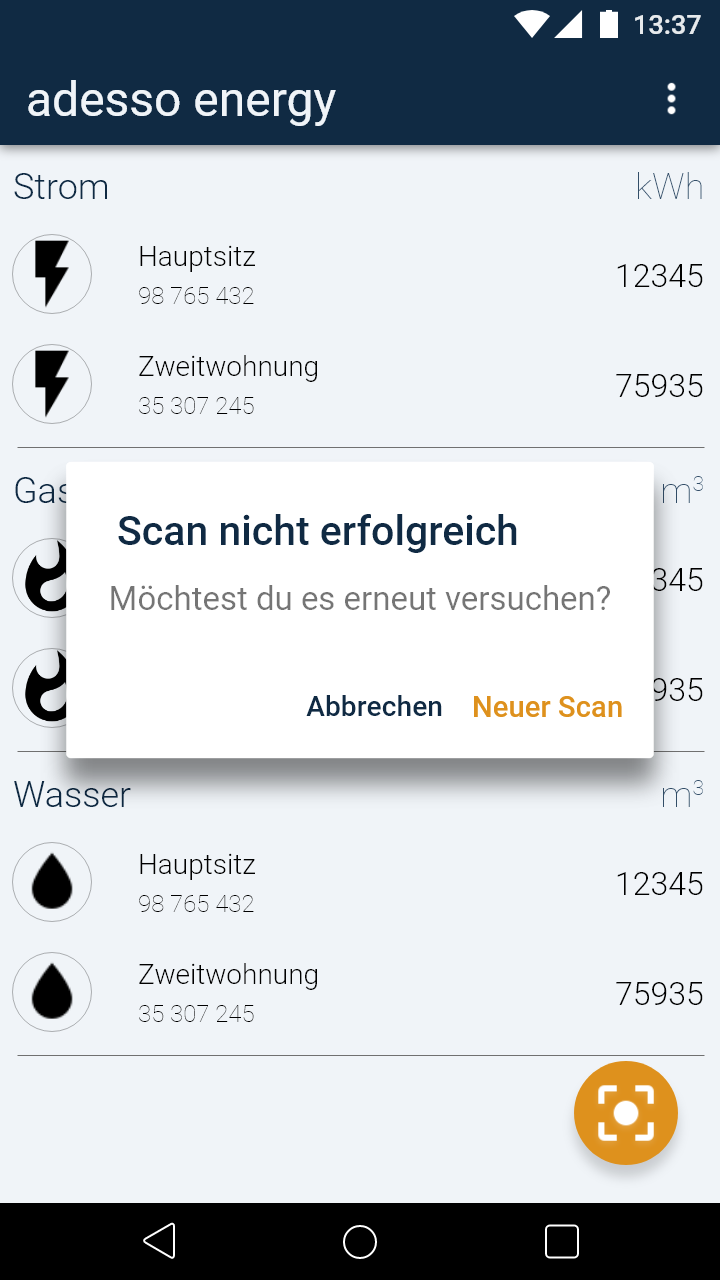
\includegraphics[scale = 0.155]{img/AndroidMockup/imageFailed} \caption{Scan fehlgeschlagen} & Wurde auf dem Bild kein Zähler erkannt, so erscheint eine entsprechende Meldung. Hier hat man die Möglichkeit, erneut ein Foto zu machen oder den Vorgang abzubrechen. \\
	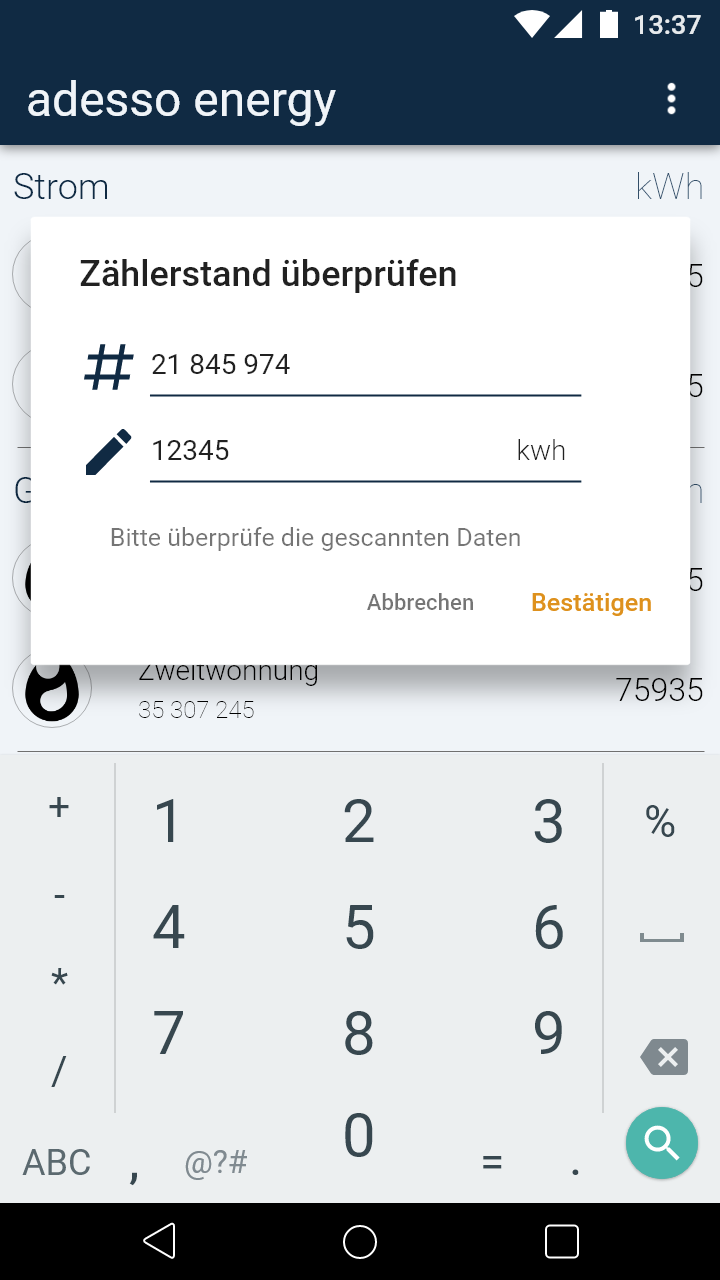
\includegraphics[scale = 0.155]{img/AndroidMockup/check} \caption{Werte überprüfen} & Wurde ein Foto erfolgreich verarbeitet, so folgt eine Überprüfung der Werte, welche von Azure erkannt wurden. Vor dem endgültigen Speichern der Werte müssen diese vom Benutzer bestätigt werden. \\ 
\end{tabularx}
\end{figure}

\begin{figure}[h]
\begin{tabularx}{\textwidth}{X  X}
	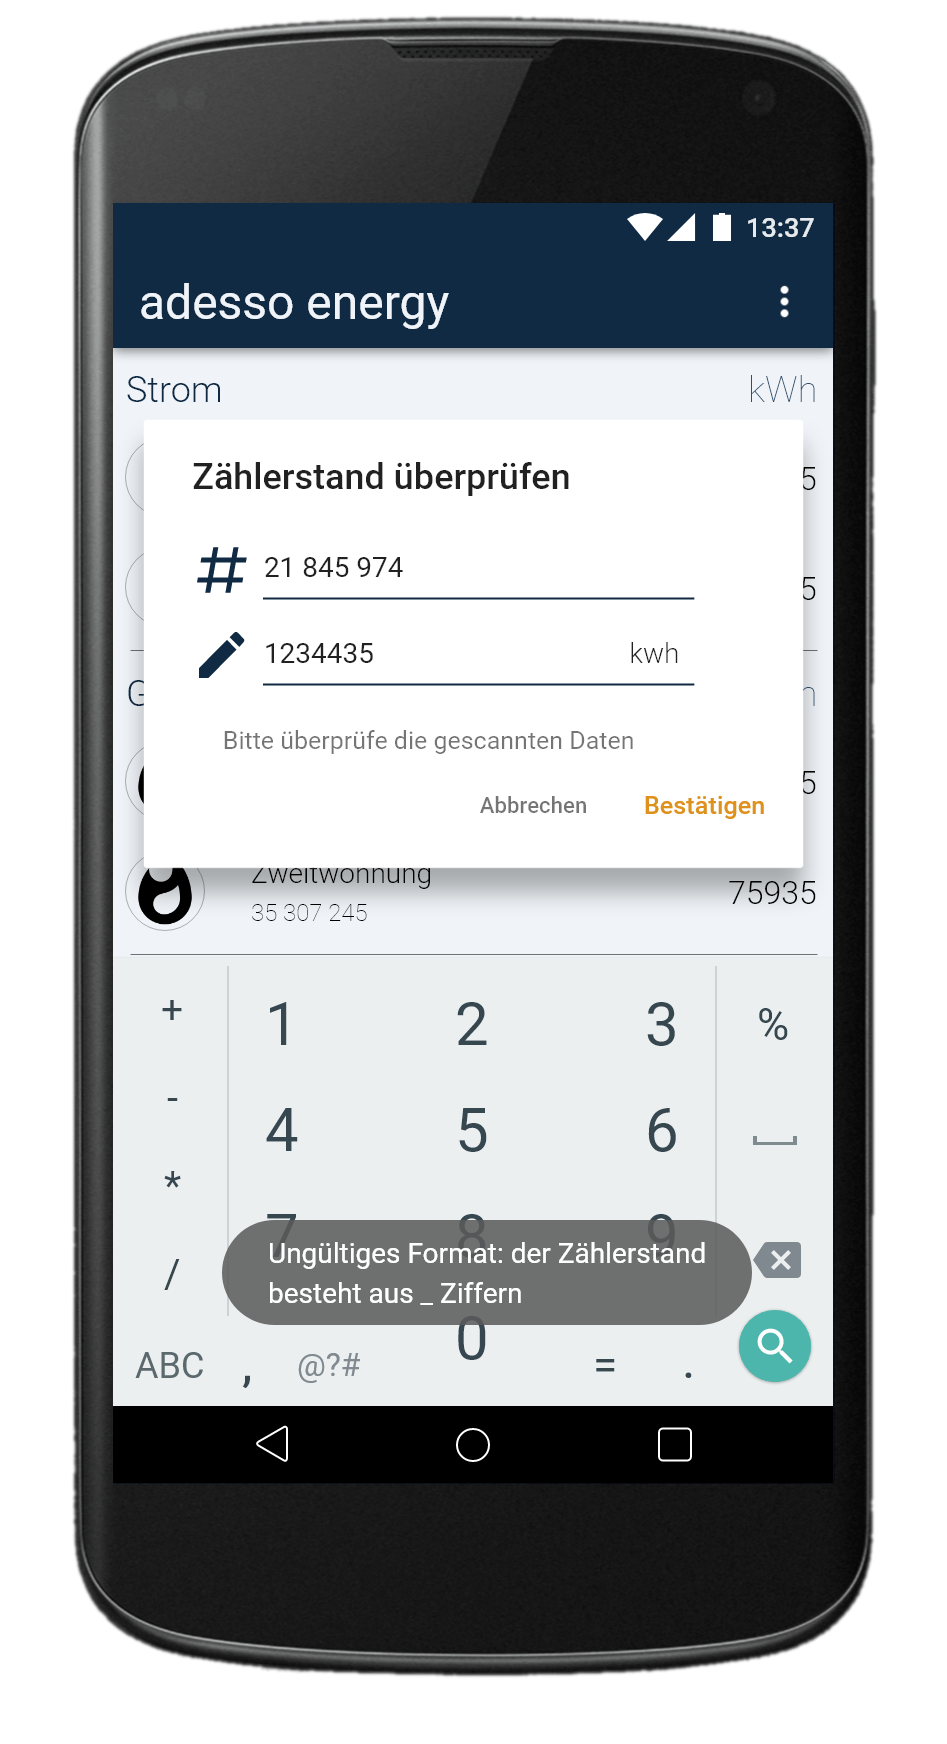
\includegraphics[scale = 0.155]{img/AndroidMockup/illegalFormatException} \caption{Falsches Zahlenformat} & Gibt man Werte in einem falschem Format ein, so erhält man eine entsprechende Meldung. \\
	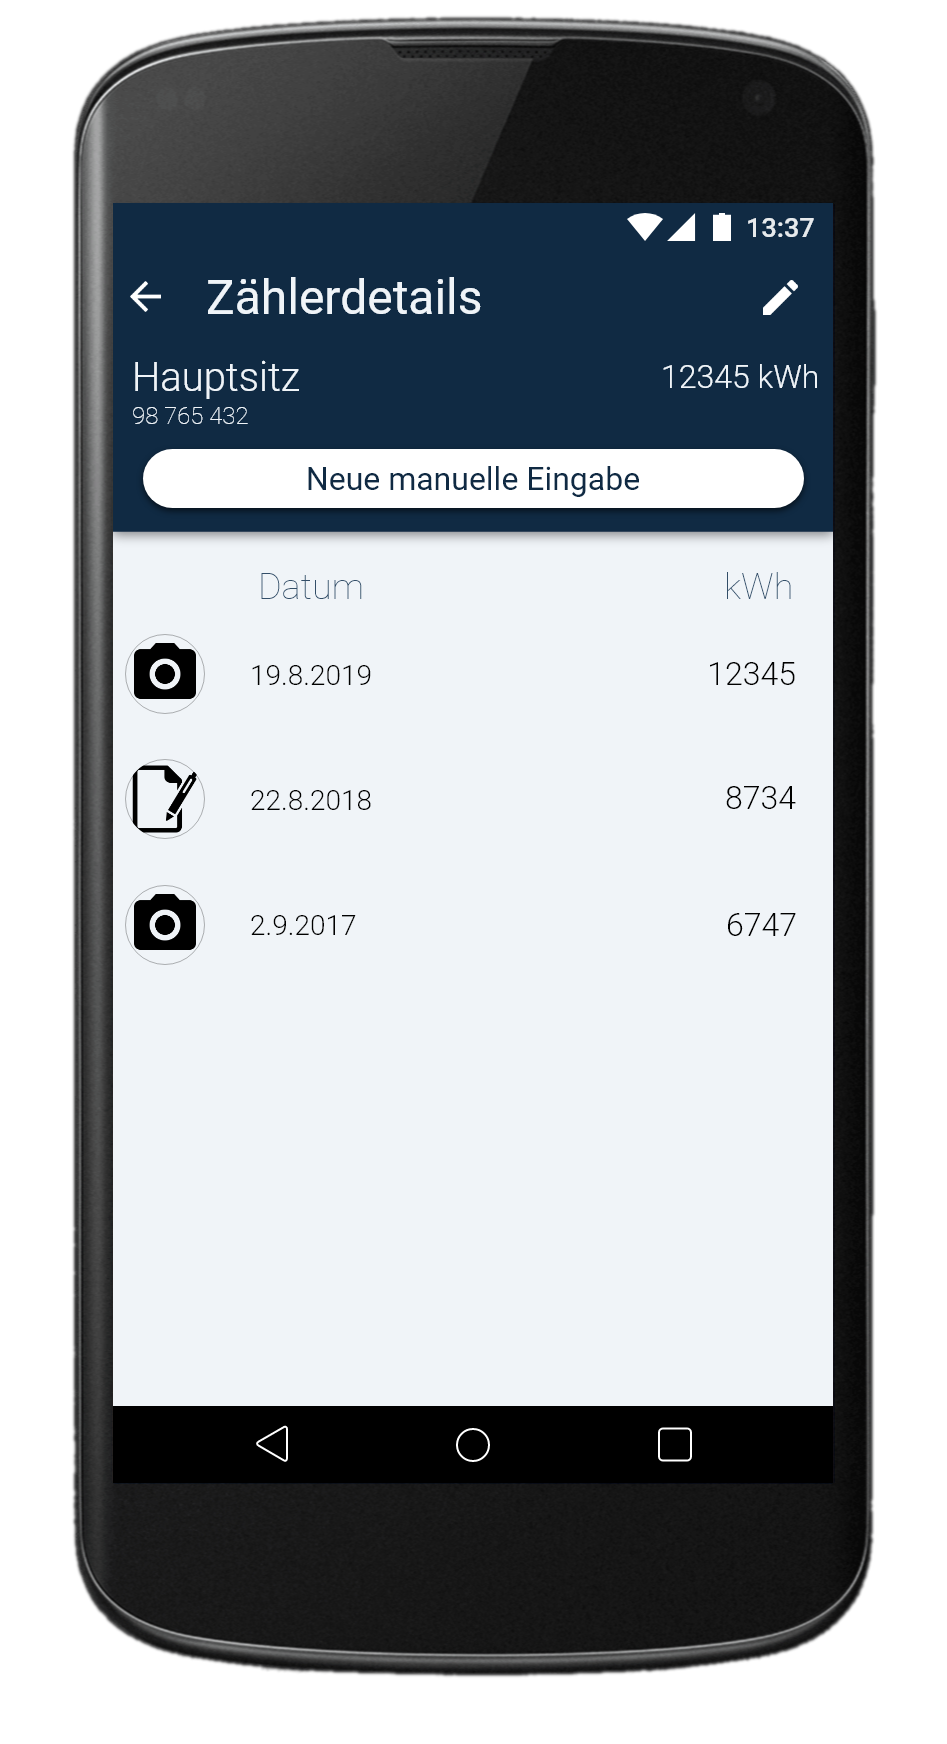
\includegraphics[scale = 0.155]{img/AndroidMockup/history} \caption{Zählerstand-Details} & Klickt man auf einen der Zähler, so sieht man die gesamte History der eingetragenen Zählerstände. Außerdem sieht man, wann der Zählerstand hochgeladen worden ist und ob dies durch eine manuelle Eingabe oder per Foto geschah. \\
\end{tabularx}
\end{figure}

\begin{figure}[h]
\begin{tabularx}{\textwidth}{X  X}
	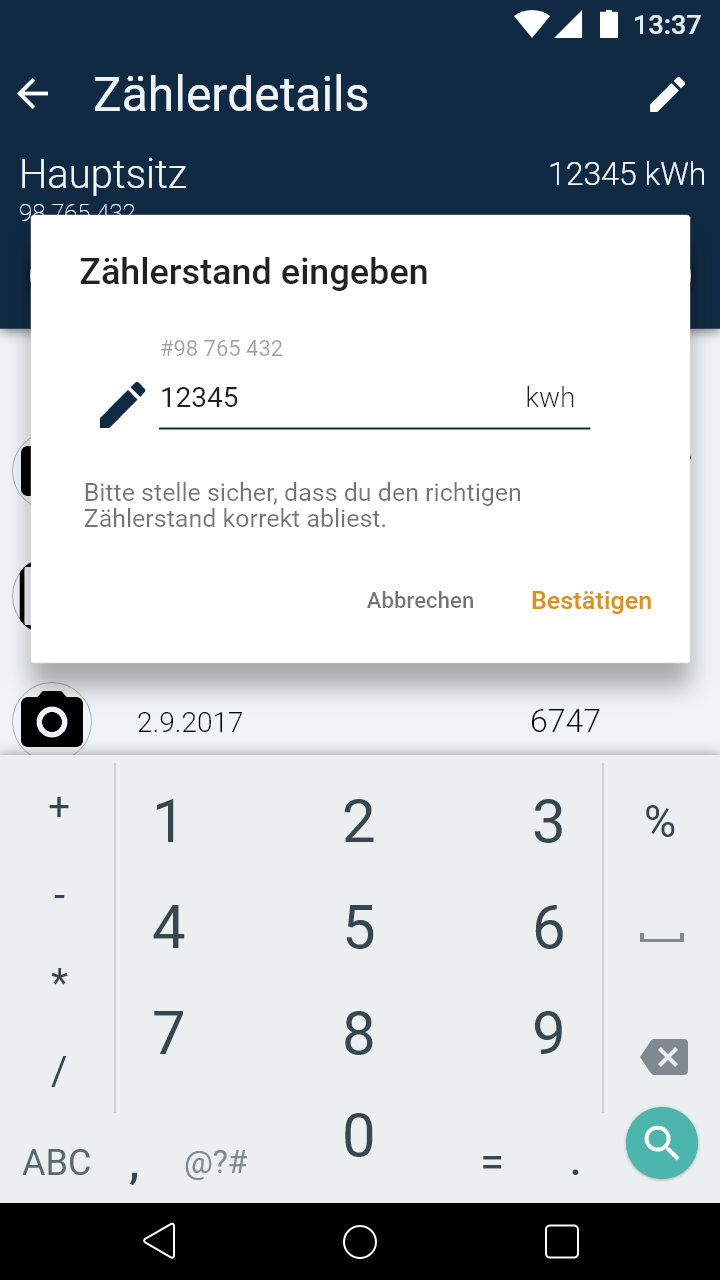
\includegraphics[scale = 0.155]{img/AndroidMockup/manuelEntry} \caption{Manueller Eintrag}&  Sobald der Zähler ausgewählt ist, hat man die Möglichkeit, manuell einen Zählerstand einzutragen. \\
	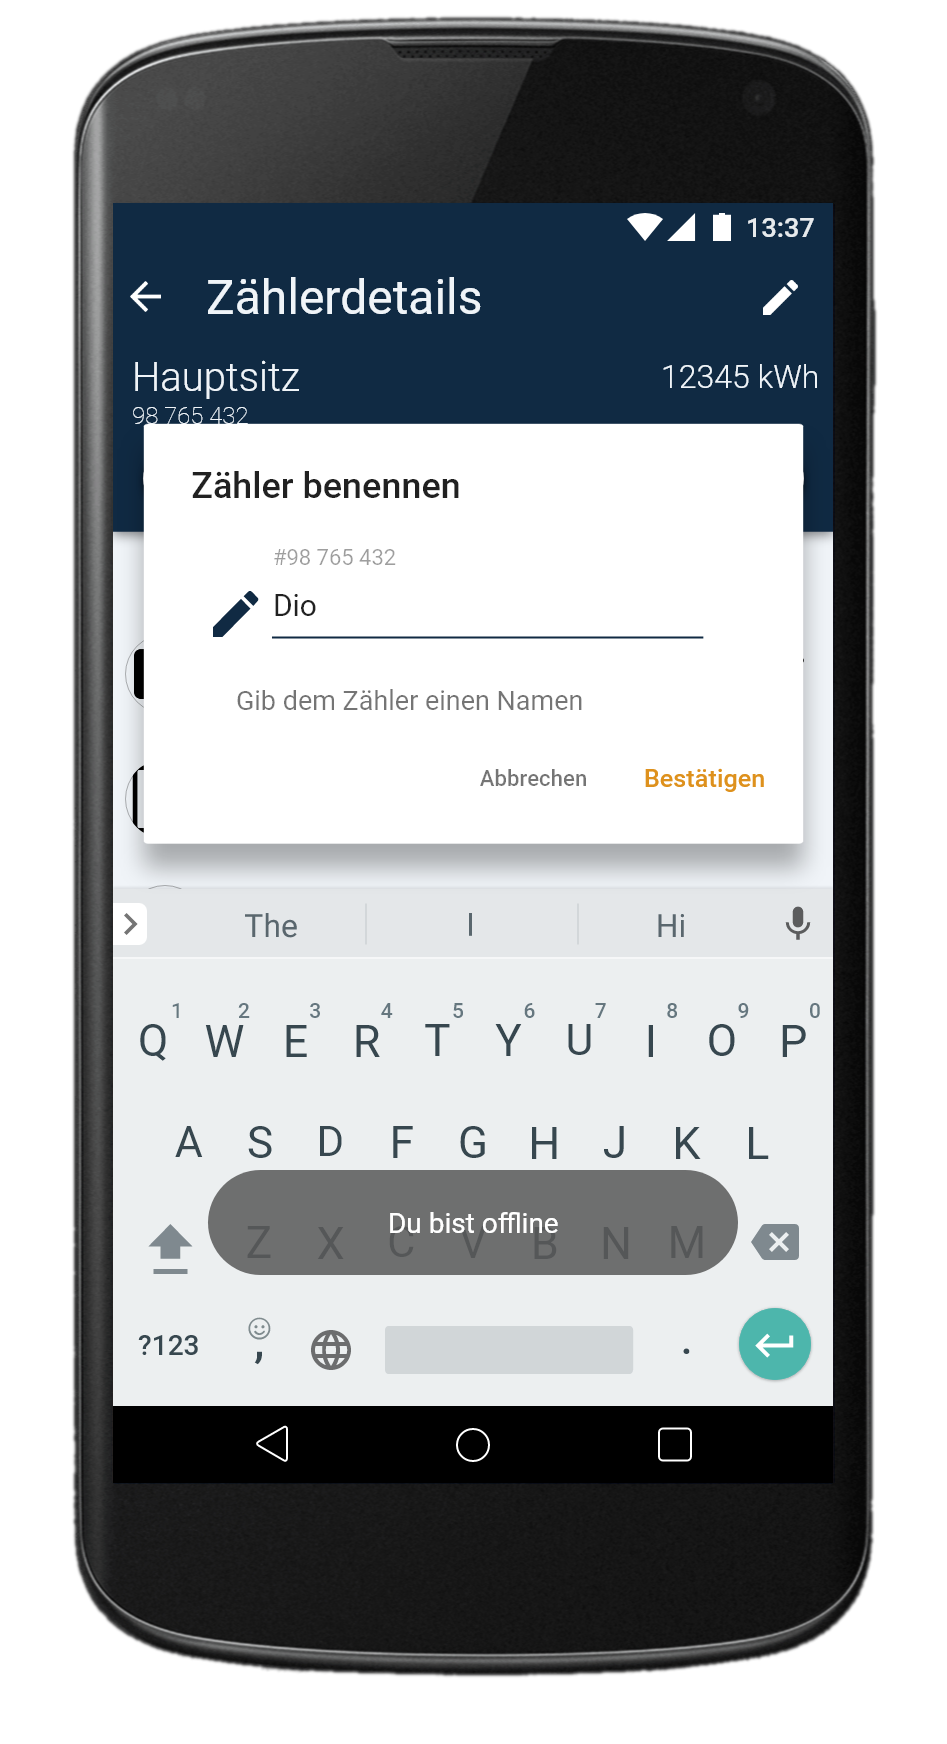
\includegraphics[scale = 0.155]{img/AndroidMockup/renameException} \caption{Offline-Meldung} & Verliert man während eines Vorganges seine Internetverbindung, so erscheint eine entsprechende Meldung und der Vorgang wird nicht durchgeführt.  \\ 
\end{tabularx}
\end{figure}

\begin{figure}[h]
\begin{tabularx}{\textwidth}{X  X}
	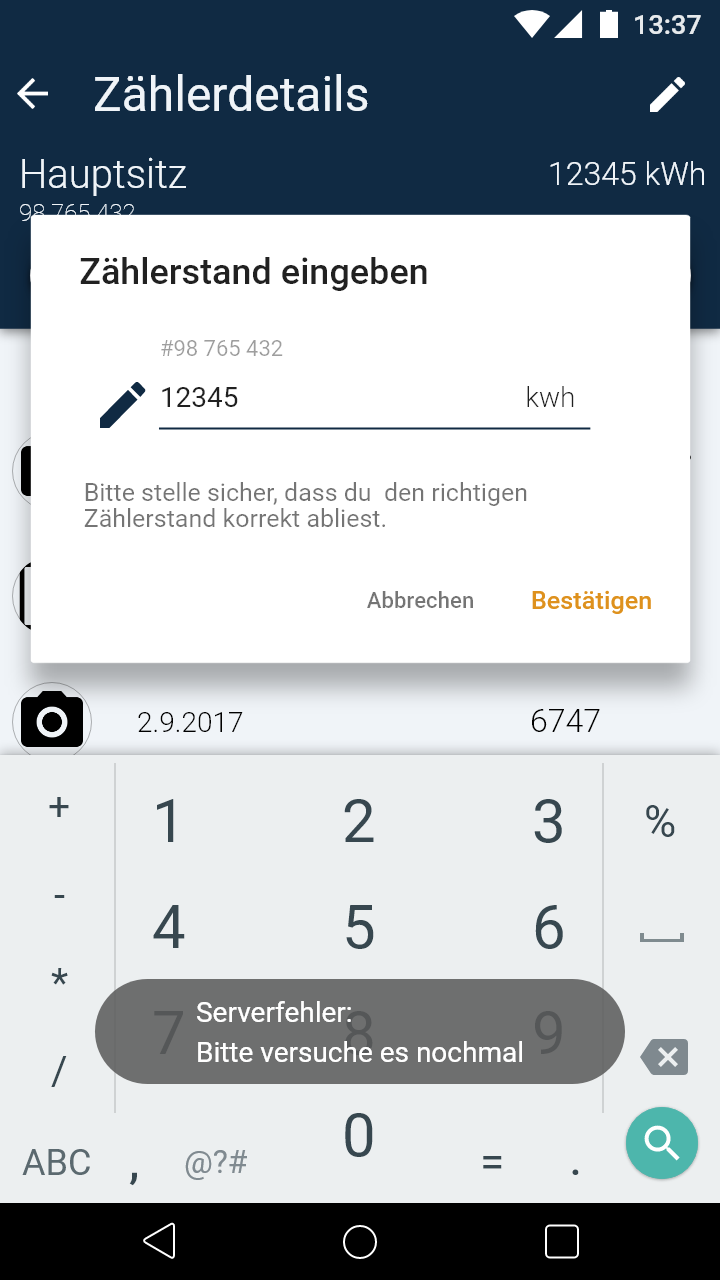
\includegraphics[scale = 0.155]{img/AndroidMockup/serverException} \caption{Serverfehler} & Falls während der Ausführung eines Vorganges ein Serverproblem geschieht, so erscheint eine entsprechende Meldung und der Vorgang wird nicht durchgeführt.\\
	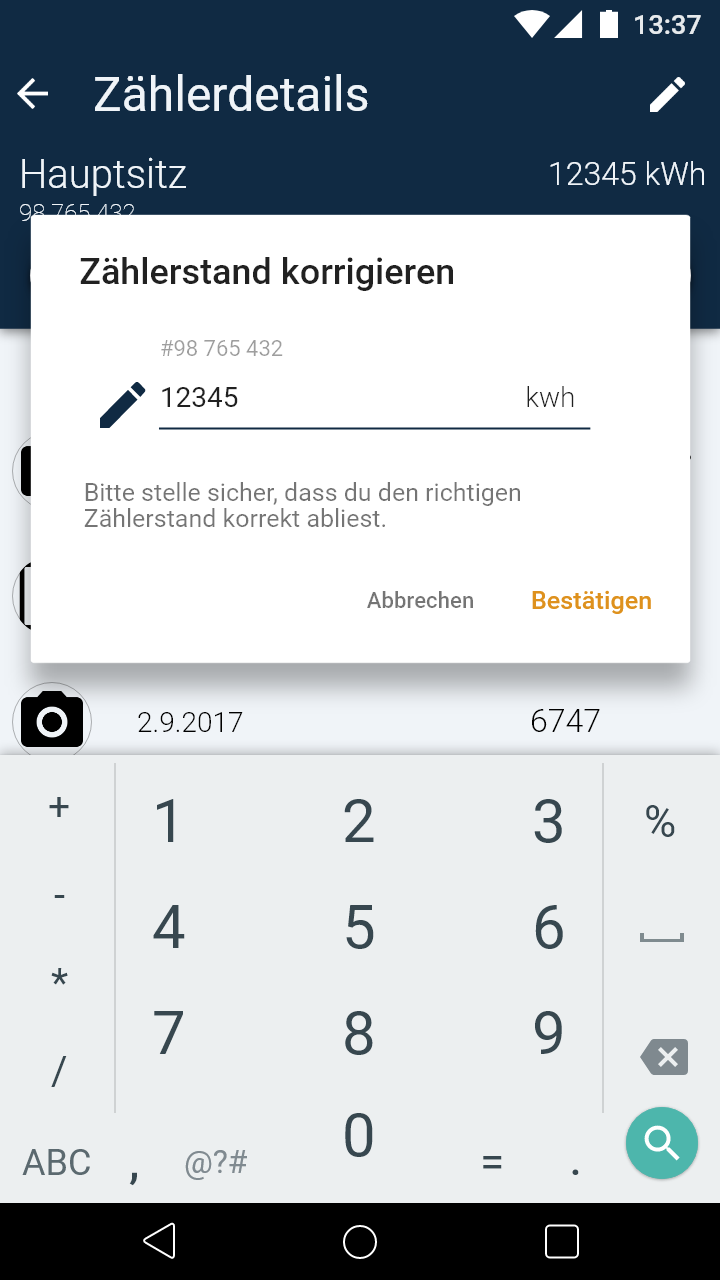
\includegraphics[scale = 0.155]{img/AndroidMockup/correct} \caption{Zählerstand korrigieren} & Wurde ein falscher Zählerstand eingetragen, so hat man nachträglich die Möglichkeit, ihn zu korrigieren.\\ 
\end{tabularx}
\end{figure}

\begin{figure}[h]
\begin{tabularx}{\textwidth}{X  X}
	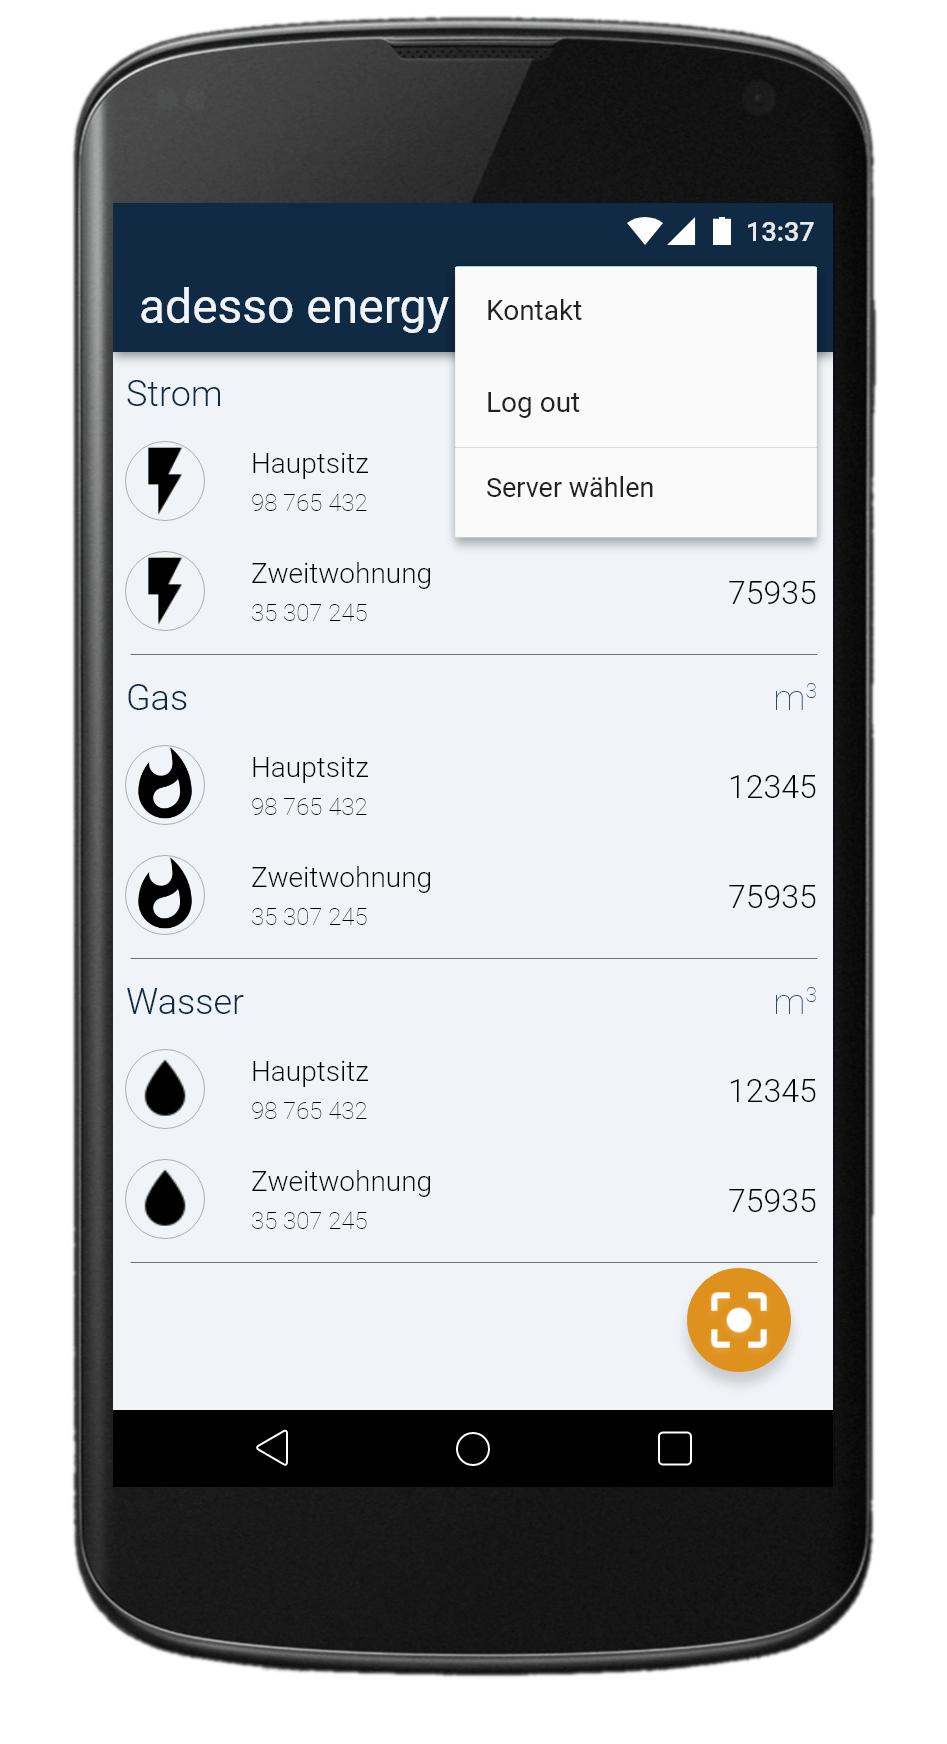
\includegraphics[scale = 0.155]{img/AndroidMockup/dropdown} \caption{Dropdown-Menü} & Man hat auf dem Startbildschirm außerdem die Möglichkeit, oben rechts ein Dropdown-Menü zu öffnen. Hier hat man die Möglichkeit, die Adresse des Servers auszuwählen, sich abzumelden, sowie Kontakt zum Support aufzunehmen. \\
	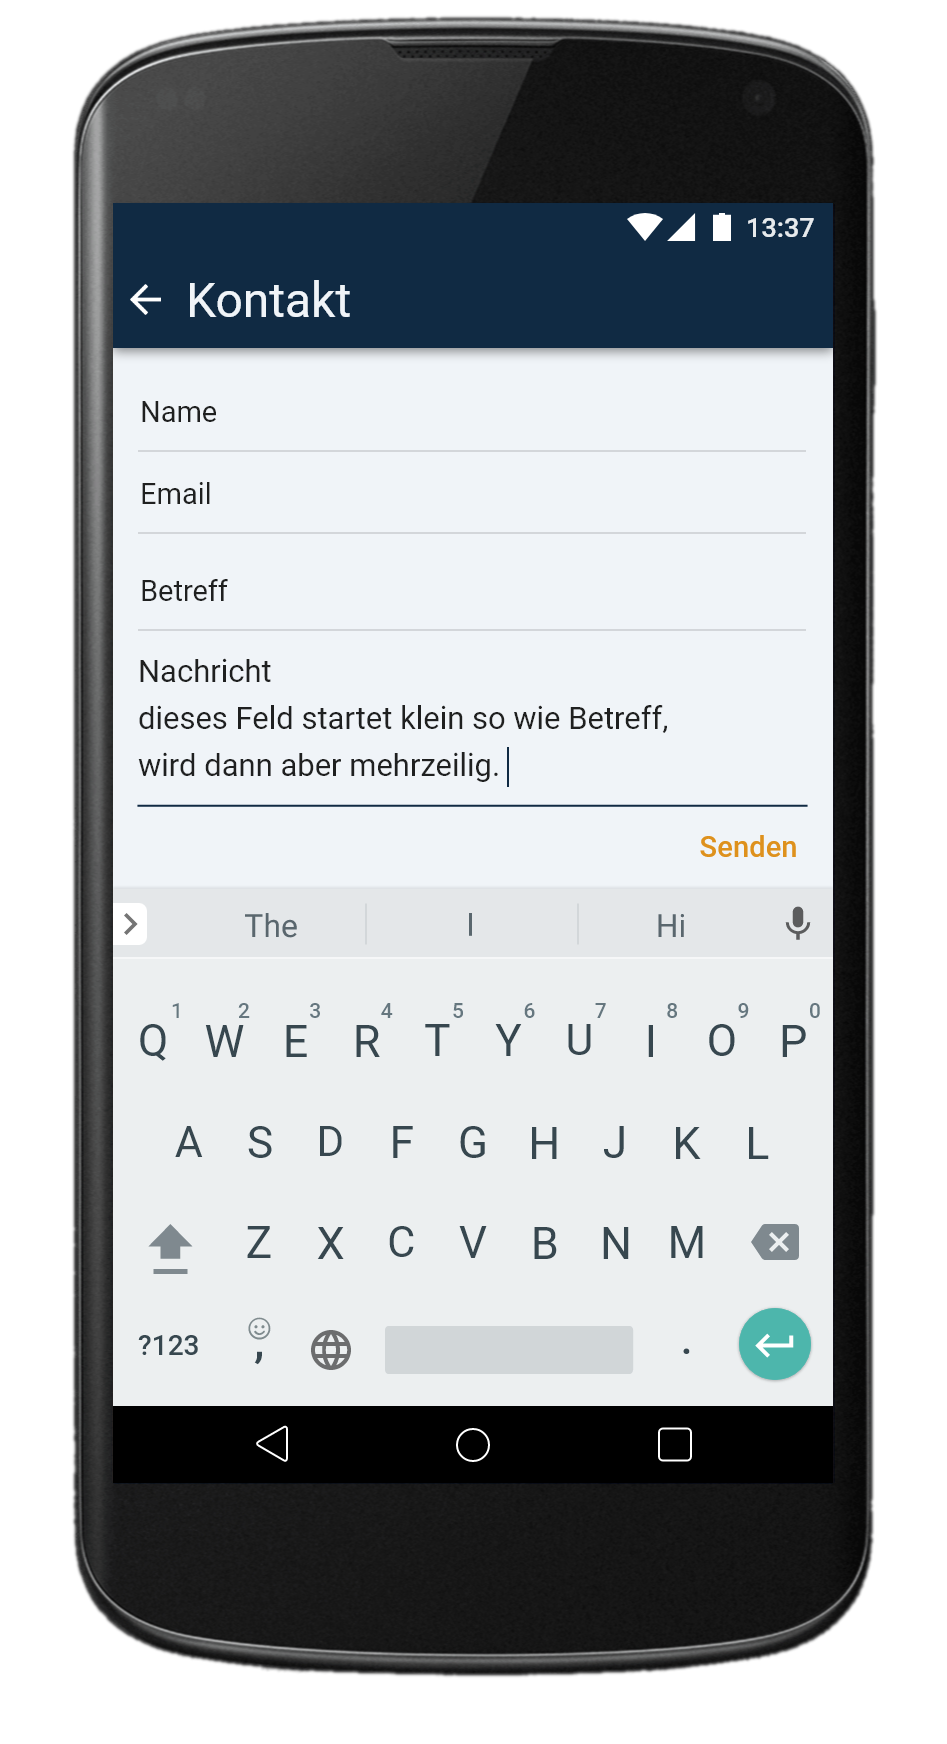
\includegraphics[scale = 0.155]{img/AndroidMockup/contact} \caption{Kontaktformular} & Sobald man sich entschieden hat, Kontakt mit dem Support aufzunehmen, erscheint ein Kontaktformular. Hier soll der Benutzer seinen Namen, seine e-Mail-Adresse, den Betreff und eine Nachricht angeben. \\ 
\end{tabularx}
\end{figure}

\begin{figure}[h]
\begin{tabularx}{\textwidth}{X  X}
	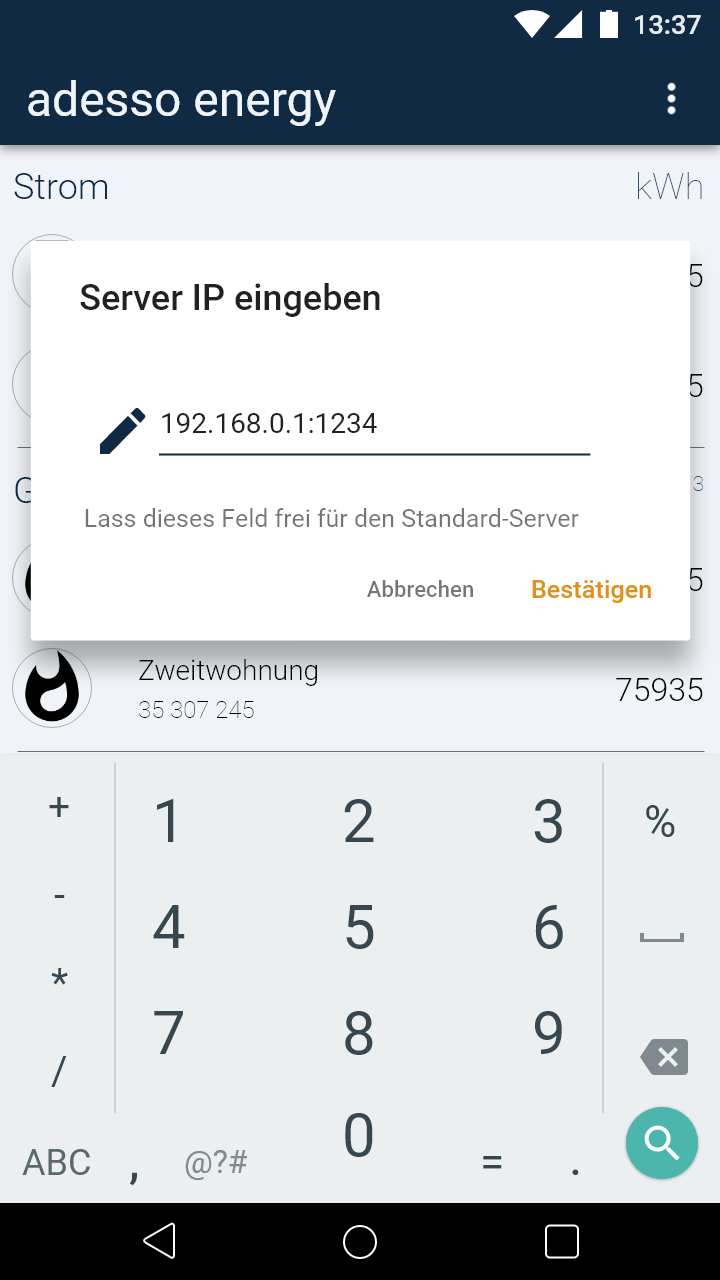
\includegraphics[scale = 0.155]{img/AndroidMockup/serverLocation} \caption{Server wählen} & Möchte man die Adresse des Servers ändern, so klickt man auf 'Server wählen'. Hier hat man die Möglichkeit, einen Servers mithilfe seiner IP-Adresse zu bestimmen und auf diesen zu wechseln. \\
	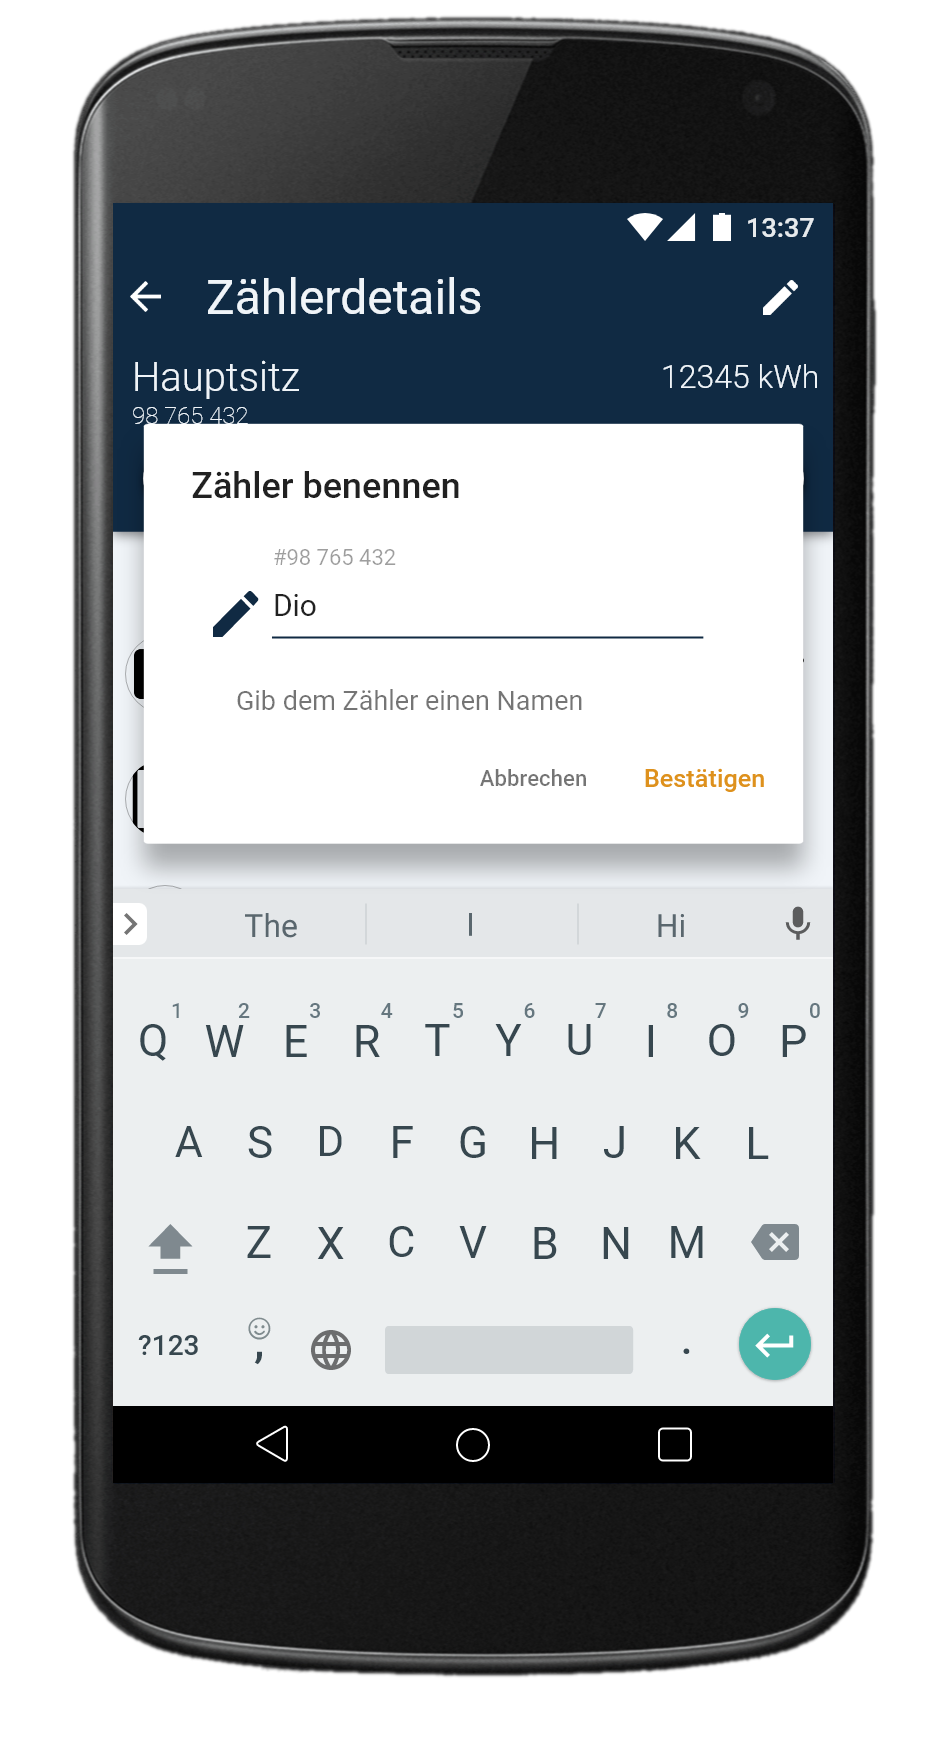
\includegraphics[scale = 0.155]{img/AndroidMockup/rename} \caption{Zähler umbenennen} & Wenn der Benutzer einen Zähler aus dem Hauptbildschirm ausgewählt hat, hat er die Möglichkeit, diesem zur einfacheren Identifikation einen Namen zuzuweisen. \\
\end{tabularx}
\end{figure}



